\documentclass[a4paper]{article}
\usepackage{cite}
\usepackage{INTERSPEECH2018}
\usepackage{amsmath}
\usepackage{color}
\newcommand{\quotes}[1]{``#1''}
\setlength{\intextsep}{10pt plus 0pt minus 3pt} %distance between floats on the top or the bottom and the text
\setlength{\textfloatsep}{10pt plus 0pt minus 4pt}%distance between two floats
\setlength{\floatsep}{10pt plus 0pt minus 2pt}%distance 
\DeclareMathOperator*{\argmax}{arg\,max}
\DeclareMathOperator*{\argmin}{arg\,min}
% \title{Cross-Lingual Knowledge Sharing For Unsupervised Feature Representation Learning}
% \title{Exploiting Speaker and Phoneme Knowledge from Resource-Rich Languages for Unsupervised Learning of Robust Feature Representation}
\title{Exploiting Speaker and Phonetic Diversity of Mismatched Language Resources for Unsupervised Subword Modeling}
% \name{Siyuan Feng, Tan Lee\thanks{This research is partially supported by a GRF project grant (Ref: CUHK 14227216) from Hong Kong Research Grants Council.}}
\name{Siyuan Feng, Tan Lee}
%The maximum number of authors in the author list is twenty. If the number of contributing authors is more than twenty, they should be listed in a footnote or in acknowledgement section, as appropriate.
\address{
  Department of Electronic Engineering, The Chinese University of Hong Kong, Hong Kong}
\email{siyuanfeng@link.cuhk.edu.hk, tanlee@ee.cuhk.edu.hk}

\begin{document}

\maketitle
% 
\begin{abstract}
This study addresses the problem of learning robust frame-level feature representation for unsupervised subword modeling in the zero-resource scenario. Robustness of the learned features is achieved through effective speaker adaptation and exploiting cross-lingual phonetic knowledge. For speaker adaptation, an out-of-domain automatic speech recognition (ASR) system is used to estimate fMLLR features for untranscribed speech of target zero-resource languages. The fMLLR features  are applied in multi-task learning of a deep neural network (DNN) to further obtain phonetically discriminative and speaker-invariant bottleneck features (BNFs). Frame-level labels for DNN training can be acquired based on two approaches:  Dirichlet process Gaussian mixture model (DPGMM) clustering, and out-of-domain ASR decoding. Moreover, system fusion is performed by concatenating BNFs extracted by different DNNs. Our methods are evaluated by ZeroSpeech 2017 Track one, where the performance is evaluated by ABX minimal pair discriminability. Experimental results demonstrate that: (1) Using an out-of-domain ASR system to perform speaker adaptation of zero-resource speech is effective and efficient; (2) Our system achieves highly competitive performance to state of the art; (3) System fusion could improve feature representation capability.
% (1). Prove the effectiveness and efficiency of using out-of-domain data in speaker adaptation of target speech; (2). Demonstrate that our system gives highly competitive performance to state of the art; (3).
\end{abstract}
\noindent\textbf{Index Terms}: zero resource, unsupervised learning, robust features, speaker adaptation, multi-task learning

\section{Introduction}
\label{sec:intro}
With the advances of deep neural network (DNN) based acoustic models (AMs) \cite{hinton2012deep} and language models (LMs) \cite{ragni2016multi}, state-of-the-art automatic speech recognition (ASR) systems have demonstrated fairly impressive performance in terms of word accuracy \cite{Saon2017,Hori2017}. Typically the training of AMs requires hundreds to thousands of hours of transcribed speech. This leads to the fact that high-performance ASR systems are available only for major languages \cite{shibata2017composite}. Even for resource-rich languages like English and Mandarin, preparing transcriptions for the available training speech requires a time-consuming task requiring considerable human effort. For many languages in the world, for which very little or no transcribed speech is available \cite{dunbar2017zero}, conventional methods of AM training can not be directly applied.

Unsupervised acoustic modeling aims at modeling speech at subword or word level, assuming that only untranscribed raw speech are available \cite{glass2012towards,kamper2015fully,thiolliere2015hybrid,feng2016exploit}. This is often referred to as the zero-resource problem. The Zero Resource Speech Challenges 2015 (ZeroSpeech 2015) \cite{versteegh2015zero} and 2017 (ZeroSpeech 2017) \cite{dunbar2017zero} precisely focused on unsupervised speech modeling without transcription. ZeroSpeech 2017 was organized to tackle two sub-problems, namely \textit{unsupervised subword modeling} (Track 1) and \textit{spoken term discovery (STD)} (Track 2). Track 1 posed a research question of how to learn a frame-level feature representation that is discriminative for subword-level units and robust to linguistically irrelevant variations, e.g., speaker change, emotion, channel, etc. 
% The feature type of unsupervised subword modeling is not constrained by challenge organizers. 
To this end, researchers proposed various feature types for comparison, such as posteriors \cite{heck2017feature,ansari2017unsupervised,shibata2017composite} and BNFs \cite{chen2017multilingual,yuan2017extracting,shibata2017composite}. 
% This paper focuses on BNFs.
Track 2 was focused on developing algorithms for discovering repeated speech patterns in audio streams. The problems concerned in the two tracks are  closely related and essential in unsupervised speech modeling. Robust feature representation is found to be preferable as compared with conventional spectral features (e.g. MFCCs) for downstream applications like STD \cite{Chen+2016}. Whilst accurate STD results could be beneficial to DNN-based supervised learning of feature representation \cite{thiolliere2015hybrid,chung2015iterative,yuan2017extracting}. The present study addresses the problem of Track 1, learning of feature representation for unsupervised subword modeling.



Speaker adaption is critical to robust acoustic modeling. It is widely acknowledged that speaker adaptive training (SAT) is effective in improving ASR performance, especially for large vocabulary tasks \cite{anastasakos1997speaker,miao2015speaker,Cui2017}. Approaches to SAT are divided into two  categories: model-based approaches, e.g., maximum likelihood linear regression (MLLR) \cite{gales1998maximum}, and feature-based approaches, e.g., feature-space MLLR (fMLLR) \cite{li2010comparison}, i-vectors \cite{saon2013speaker}, speaker codes \cite{xue2014fast}, and other appending features \cite{Xie2017}.
 % \cite{seltzer2013investigation,Xie2017}. 
All of these methods are based on the assumption that speech transcription and/or speaker identity information are available. In the zero-resource case, Heck et al. proposed to estimate fMLLRs based on frame-level cluster labels that were obtained by a Dirichlet process Gaussian mixture model (DPGMM) algorithm \cite{heck2017feature}. The cluster labels are regarded as pseudo transcriptions for the target speech, which facilitate context-dependent GMM-HMM (CD-GMM-HMM) acoustic modeling with fMLLR features. This system demonstrated the best performance among all submitted systems in the ZeroSpeech 2017. 
Zeghidour et al. regards speaker adaptation as a problem of disentangling speaker information from phoneme information in speech \cite{Zeghidour+2016}. They proposed to train subword and speaker same-different tasks within a triamese network, and demonstrated the effectiveness of disentanglement between  these two types of information. This approach assumes availability of subword same-different supervision, which could be derived from STD results.
% , which may be obtained via an STD system.

For major languages, high-performance ASR systems can be trained with large-scale speech corpora that cover hundreds of speakers \cite{paul1992design,LeeLoChingEtAl2002}. The richness of speaker diversity and linguistic variation in these out-of-domain corpora could be leveraged for learning robust feature representations in the zero-resource scenario. In \cite{shibata2017composite}, Shibata et al. made use of a Japanese ASR system to estimate fMLLR features and demonstrated very good performance in Track 1 of ZeroSpeech 2017. 
%-----%
In the present study, we propose a framework of unsupervised learning of multilingual bottleneck features. To facilitate fMLLR-based SAT with untranscribed speech, frame-level labels are generated either by DPGMM clustering or using the state-level alignment information from an out-of-domain ASR system. BNFs are obtained from a multi-task learning DNN (MTL-DNN), which is trained with these two types of labels. As an alternative approach, the BNFs can be obtained directly from the same out-of-domain AMs. We also investigate on the efficacy of system fusion by concatenating the BNFs obtained from different DNNs.
%-----%
% Motivated by this, 
% % These corpora usually contain tens or hundreds of speakers covering both male and female \cite{paul1992design,LeeLoChingEtAl2002}. 
% % This drives us to investigate on whether and how out-of-domain transcribed and speaker annotated speech can be efficiently exploited  to model speaker variation embedded in target speech, in order to learn features that are able to de-emphasize speaker identity. 
% our proposed methods can be summarized as in two parts. In the first part, we incorporate fMLLR-based speaker adaptation in unsupervised multilingual bottleneck feature (BNF) learning framework \cite{chen2015parallel}, where fMLLR features for in-domain speech are estimated by AM of an out-of-domain ASR system. Apart from the DPGMM frame labeling method 
% % clustering based frame label acquisition 
% proposed in \cite{chen2015parallel}, we propose to use an out-of-domain ASR system to decode in-domain speech and generate HMM state alignment as the second type of frame labels.
% % Frame labels needed for neural network (NN) training are obtained from DPGMM clustering results, as discussed in \cite{chengexploration}. In addition, we propose to use an out-of-domain ASR system to decode in-domain speech and generate frame-level HMM state alignment as the second type of frame labels. 
% A multi-task learning DNN (MTL-DNN) is then trained with two types of labels and used to extract BNFs as the learned representation for evaluation. In the second part, an out-of-domain DNN-HMM AM directly feeds forward in-domain speech and generate BNFs for evaluation. Furthermore, we also investigate on the efficacy of system fusion by concatenating BNFs extracted by multiple systems.
%------------%
% The feature type of unsupervised subword modeling is not constrained by challenge organizers. Researchers proposed various feature types for comparison such as posteriors \cite{heck2017feature,ansari2017unsupervised,shibata2017composite} and BNFs \cite{yuan2017extracting,chen2017multilingual,shibata2017composite}. This paper focuses on BNFs.
%------------%
% A multi-task learning DNN (MTL-DNN) is trained with fMLLRs of zero-resource languages and multiple frame-level label prediction tasks.

\section{Speaker adaptation with out-of-domain data}
\label{sec:SAT}

Feature-based speaker adaptation, e.g., fMLLR, is an effective approach to improving robustness of speech features. In the case of zero resource, we propose to leverage out-of-domain transcribed and speaker-annotated speech from a resource-rich language to model the speaker variation in target speech. Given the out-of-domain data, context-dependent GMM-HMM (CD-GMM-HMM) AMs are trained with raw spectral features. The models are used to forced-align the training data to provide supervision for vocal tract length normalization (VTLN) \cite{kim2004using}, linear discriminant analysis (LDA) \cite{haeb1992linear}, maximum likelihood linear transforms (MLLT) \cite{gales1999semi} and fMLLR estimation \cite{povey2012basis}. Subsequently CD-GMM-HMM models with SAT (CD-GMM-HMM-SAT) are trained, and used to estimate fMLLR transforms for the target zero-resource speech utterances. It is noted that the estimated fMLLR features of target speech can be used directly for subword modeling.
The fMLLR features are expected to serve a better baseline than raw spectral features like MFCCs for subsequent feature representation learning and system building. 

\section{Frame labeling}
\label{sec:frame_labeling}
Frame labeling is an essential step to prepare the target speech utterances for DNN based subword discriminative modeling. While frame labels are not needed in some of the DNN models like autoencoders (AEs), there were studies suggesting that AEs might not be a good approach to improving acoustic features \cite{renshaw2015comparison}. In this study,  two frame-labeling approaches are investigated, namely, DPGMM clustering and out-of-domain ASR decoding. 

% \subsection{DPGMM clustering}
DPGMM is a non-parametric Bayesian extension to GMM, in which a Dirichlet process prior replaces the vanilla GMM \cite{chang2013parallel}. One advantage of the DPGMM clustering algorithm is that the cluster number does not need to be pre-defined.  This makes the algorithm very suitable for the problem of unsupervised acoustic modeling, as the number of basic speech units is unknown for a zero-resource language. Previous studies showed successful application of DPGMM to unsupervised word clustering \cite{kamper2014unsupervised}, frame-level feature clustering for subword discriminative modeling \cite{chen2015parallel} and unsupervised fMLLR-based speaker adaptive training \cite{Heck+2016,heck2017feature}.

Let us consider $M$ zero-resource languages. For the $i$-th language, frame-level fMLLR features, estimated as described in Section \ref{sec:SAT}, are denoted as $\{\bm{x_1^{i}, x_2^{i}, \ldots, x_L^{i}}\}$, where $L$ is the number of frames in the utterance. By applying DPGMM clustering, $K$ Gaussian components are obtained to represent $K$ clusters of frame-level features. The frame-level labels $\{l_1^{i}, l_2^{i}, \ldots, l_L^{i}\}$, are obtained by
\begin{equation}
\label{eqt:dpgmm_inference}
l^{i}_{t} = \argmax_{1 \le k \le K} p_{i,k},
\end{equation}
where $p_{i,k}=P(k | \bm{x_{t}^{i}})$ denotes the posterior probability of $\bm{x_{t}^{i}}$ with respect to the $k$-th Gaussian component.

A Metropolis-Hastings based split/merge sampler is adopted for the inference of DPGMM parameters \cite{chang2013parallel}, following other studies on ZeroSpeech Challenges \cite{heck2017feature,chen2015parallel}. 
% We refer to 

% \subsection{Frame labeling by ASR decoding}
Frame labeling can also be done with an out-of-domain ASR system, which is typically trained with a large amount of transcribed speech in a resource-rich language. The AM in such ASR system provides fine-grained speech representation of the language. Given an input speech utterance of the target zero-resource language, the out-of-domain ASR system can be applied to assign a language-mismatched state label to each frame of the utterance. It must be noted that the result of ASR decoding depends on the relative weighting of AM and LM. In our application, the LM carries a a very small weight, such that the acquired frame labels mainly reflect the acoustic properties of target speech. 
 % an out-of-domain AM's HMM states. 
% \section{title}
\section{Multi-task learning for BNFs}
\label{sec:MTL}
After obtaining frame-level labels for the training utterances of target speech, a DNN is trained with the fMLLR features, with the goal of extracting BNFs for subword modeling. BNFs have been shown to provide a compact and phonetically-discriminative representation, and suppress linguistically-irrelevant variation, e.g., speaker identity, of the input speech \cite{grezl2009investigation}. In this study, a multi-task learning (MTL) DNN is adopted in order to leverage the phonetic diversity in different speech tasks and different languages \cite{caruana1998multitask}. The proposed DNN architecture is shown as in Figure \ref{fig:mtl}.
\begin{figure}[tbp]
\centering
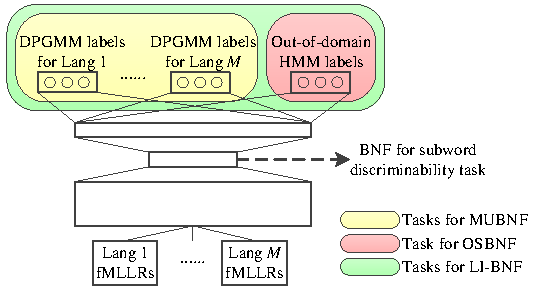
\includegraphics[width = 0.85 \linewidth]{MTL_tnr_embed.pdf}
\caption{DNN for extracting LI-BNF, MUBNF and OSBNF}
\label{fig:mtl}
\end{figure}
The DNN supports a total of $M+1$ learning tasks, which correspond to the $M$ target zero-resource languages and the out-of-domain ASR. For the zero-resource language tasks, the frame labels are obtained by applying DPGMM clustering to training speech of the $M$ target languages, while the out-of-domain ASR system generates an additional frame label. The hidden layers of the DNN, including a low-dimensional linear bottleneck layer, are shared across all tasks, while the soft-max output layers are task-specific. After multi-task training, the DNN is used to generate language-independent BNFs (LI-BNFs) for subword discriminability task.

It must be noted that one could also choose either the $M$ language-dependent DPGMM label prediction tasks or the additional out-of-domain label prediction task for DNN training. As illustrated in Figure \ref{fig:mtl}, the BNFs generated by these sub-tasks are denoted as multilingual unsupervised BNFs (MUBNFs) and the out-of-domain supervised BNFs (OSBNFs).

There are two main reasons why the MTL approach is adopted. First, there are two types of frame labels being investigated in this work, namely the DPGMM cluster labels and ASR decoding labels. The two tasks of label prediction are believed to be positively correlated and therefore are expected to benefit from MTL \cite{caruana1998multitask}. Second, one of the requirements of ZeroSpeech 2017 is that the learned feature representations for all target languages be generated by exactly the same system input and output. The idea of training a separate DNN for each target language would not satisfy the requirement\footnote{\label{footnote:ffnn}Although better  performance was found by language-specific BNFs during our experiments, we do not report it in this paper.}. 

\section{System fusion}
If there are multiple systems developed for feature representation learning which provide complementary information, fusion of these systems is expected to further improve the feature representation capability.
System fusion can be done at either model level or output level. MTL is considered a kind of model-level fusion. LI-BNFs, as described in Section \ref{sec:MTL}, can be considered as model-level fusion of MUBNFs and OSBNFs. Output-level system fusion can be realized by concatenating multiple feature representations. In this study, the effectiveness of output-level fusion is validated by:
\begin{itemize}
\item[1.] Concatenating language-mismatched BNFs (LM-BNFs), which are obtained from the out-of-domain DNN-HMM AM, and LI-BNFs (LM-BNF + LI-BNF);
\item[2.] Concatenating LM-BNFs, MUBNFs and OSBNFs (LM-BNF + MUBNF + OSBNF).
\end{itemize}
% concatenating language-mismatched BNFs (LM-BNFs), which are obtained from the out-of-domain DNN-HMM AM, and LI-BNFs, or concatenating LM-BNFs, MUBNFs and OSBNFs. 
% The effectiveness   of concatenating BNFs extracted by both in-domain and out-of-domain trained DNNs is 
% Both model-level and output-level system fusion methods are explored in this work.

\section{Experiments}

\subsection{Dataset and evaluation metric}
% To evaluate our methods of unsupervised feature representation learning, and to facilitate direct comparison between our system and state-of-the-art works by other researchers, the 
Experiments are carried out with development data of ZeroSpeech 2017 Track one \cite{dunbar2017zero}.
% , \textit{unsupervised subword modeling} task \cite{dunbar2017zero}. 
The development data consists of three languages, i.e., English, French and Mandarin. Each language contains separate training and test sets of untranscribed speech. Speaker identity information is made publicly known for train sets while unknown for test sets. Test sets are organized into subsets of differing utterance length (1s, 10s and 120s). Detailed information of the dataset is listed in Table \ref{tab:zr17_data}.

\begin{table}[htbp]
\renewcommand\arraystretch{0.8}
\centering
\caption{Development data in ZeroSpeech 2017 Track one}
\resizebox{0.65 \linewidth}{!}{%
\begin{tabular}{lcc|c}      
% \hline      
\toprule
 & \multicolumn{2}{c|}{ Training} & Test \\
\midrule
 & Duration  & \#speakers  & Duration\\
% \hline
\midrule
English & $45$ hrs & $60$ & $27$ hrs\\
French & $24$ hrs & $18$ & $18$ hrs\\
Mandarin & $2.5$ hrs & $8$ & $25$ hrs\\
% Training hours:  & $19.3$ & $81.5$ & $105.3$ \\
% Test hours:& $0.6$ & $0.7$ & $5.9$ \\
% Basic acoustic unit:  & Phone & Phone & Initial-Final \\
% \#basic units (inc. sil):& $33$ & $87$ & $61$ \\
% \#tied CD-HMM states:& $2462$ & $3431$ & $2386$ \\ 
% Lexicon size:& $ $ & $ 133K$& $ $ \\
% $\#$ Phonemes: &$43$& $46$&$ 29$& $44$& $38$\\
% \hline
\bottomrule
\end{tabular}%
}
\label{tab:zr17_data}
\end{table}

The evaluation metric of ZeroSpeech 2017 is ABX subword discriminability. Briefly speaking, the ABX task is to decide whether $X$ belongs to $x$ or $y$ if $A$ belongs to $x$ and $B$ belongs to $y$, where $A$, $B$ and $X$ are three speech segments, $x$ and $y$ are two phonemes that differ in the central sound (e.g., \quotes{beg}-\quotes{bag}). 
% Dynamic time warping (DTW) is used to measure the dissimilarity between each pair of speech segments, the underlying frame-level dissimilarity is allowed to be defined by participants. In this paper, cosine distance is selected as recommended by challenge organizers. 
Each pair of segments $A$ and $B$ are generated by the same speaker. 
% Depending on whether the segment $X$ belongs to the same speaker as $A$($B$), 
ABX error rates for \textit{within-speaker} and \textit{across-speaker} are evaluated separately, depending on whether $X$ and $A(B)$ belong to the same speaker.
Dynamic time warping (DTW) and cosine distance are used to measure segment-level and frame-level dissimilarity, respectively.
% More details can be found on \cite{dunbar2017zero}.

\subsection{Out-of-domain ASR system}
\label{subsec:ood_asr}
A Cantonese ASR is selected as the out-of-domain ASR system. 
% We choose Cantonese as a resource-rich language for two main reasons. First, Cantonese is different from any languages in ZeroSpeech 2017 development data, in line with the spirit of unsupervised learning. 
% It is worth noting that although both  Mandarin and Cantonese belong to Chinese, these two languages are mutually unintelligible. 
% A well-developed Cantonese ASR system has been trained in our previous work, which facilitates the system design in this work. 
The ASR is trained with CUSENT, a read speech corpus developed by The Chinese University of Hong Kong \cite{LeeLoChingEtAl2002}. There are $20,378$ training utterances from $34$ male and $34$ female speakers, with a total of $19.3$ hours speech. Kaldi \cite{povey2011kaldi} is used to train two AMs, one is CD-GMM-HMM-SAT, the other is DNN-HMM.  Target labels for DNN-HMM training are state alignments of CUSENT training data generated by CD-GMM-HMM-SAT model.
% DNN-HMM is trained with state alignments of CUSENT data generated by CD-GMM-HMM-SAT model.
% and a syllable trigram language model. 
Input features are $40$-dimensional fMLLRs for CD-GMM-HMM-SAT, or fMLLRs by splicing with context size $\pm 5$ for DNN-HMM. The fMLLR features are generated by performing VTLN towards $39$-dimensional MFCCs+$\Delta$+$\Delta\Delta$, and processed by splicing with context size $\pm 3$ to estimate $40$-dimensional LDA and MLLT, followed by fMLLR estimation. The total number of CD-HMM states are $2462$. DNN-HMM has $7$ hidden layers, with dimensions $440$-$1024\times 5$-$40$-$1024$-$2462$, and sigmoid activation function except for the $40$-dimensional linear bottleneck layer.
% . Sigmoid  is chosen as nonlinear activation function.
% The nonlinear function is Sigmoid, except for the linear bottleneck layer. 
A syllable trigram language model trained with transcriptions of CUSENT training data is used during decoding. The language model is trained with SRILM toolkit \cite{Stolcke02srilm--}.
\begin{table*}[htbp]
\renewcommand\arraystretch{0.9}
\centering
\caption{ABX error rate ($\%$) on the proposed methods, MFCC and state of the art of ZeroSpeech 2017}
\resizebox{1 \linewidth}{!}{%
\begin{tabular}{lccc|ccc|ccc|c||ccc|ccc|ccc|c||c}      
% \hline      
\toprule
 & \multicolumn{10}{c||}{ Within-speaker} & \multicolumn{10}{c||}{ Across-speaker} & Avg.\\
\midrule
 & \multicolumn{3}{c|}{ English} & \multicolumn{3}{c|}{ French} & \multicolumn{3}{c|}{Mandarin}& Avg.&\multicolumn{3}{c|}{ English} & \multicolumn{3}{c|}{ French} & \multicolumn{3}{c|}{Mandarin} & Avg.\\
 & 1s & 10s & 120s & 1s & 10s & 120s & 1s & 10s & 120s && 1s & 10s & 120s & 1s & 10s & 120s & 1s & 10s & 120s &\\ 
% \midrule
%  & Duration & \#speakers  & Duration\\
% \hline
\midrule
Baseline (MFCC) \cite{dunbar2017zero}& $12.0$ & $12.1$ & $12.1$ & $12.5$ &$12.6$ &$12.6$ &$11.5$ &$11.5$ & $11.5$&$12.0$ & $23.4$& $23.4$& $23.4$& $25.2$&$25.5$ &$25.2$ &$21.3$ &$21.3$ &$21.3$ & $23.3$ & $17.7$\\

fMLLR & $8.0$ & $8.2$ &$ 7.3$ & $10.3$ & $10.3$ & $9.1$ & $9.3$ &$ 9.3$ &$ 8.4$ & $8.9$ & $13.4$ & $12.0$ & $11.3$ & $17.2$ & $15.8$ & $14.8$ &$ 10.7$ & $10.2$ & $9.4$ & $12.8$ & $10.8$ \\

MUBNF & $7.4$ & $6.9$ & $6.3$ & $9.6$ & $9.0$ & $8.1$ & $9.8$ & $8.8$ & $8.1$ & $8.2$ & $10.9$ & $9.5$ & $8.9$ & $15.2$ & $13.0$ & $12.0$ & $10.5$ & $8.9$ & $8.2$ & $10.8$ & $9.5$\\

OSBNF & $7.2$ &$7.1$&$6.3$&$10.2$&$9.7$& $8.7$&$9.1$ &$8.6$ &$7.6$ & $8.3$ & $10.0$& $9.7$&$8.6$&$13.9$&$13.4$&$11.6$&$9.0$&$8.4$&$7.5$&$10.2$&$9.3$\\

LI-BNF & $6.9$ & $6.6$ & $6.1$ & $9.5$ & $9.2$ & $8.4$ & $9.2$ &$ 8.5$ & $7.9 $&$ 8.0$ &$ 10.0 $& $\bm{8.9}$ & $\bm{8.2}$ & $14.3 $& $12.9$&$ 11.5$&$ 9.5$& $8.5$& $7.7$ & $10.2$ &$9.1$\\

LM-BNF & $7.2$ & $6.8$& $6.1$& $9.6 $& $9.0$ & $8.0$&$ 8.7$& $7.6$& $6.8$& $7.8$ &$ 10.6$& $9.6$& $8.7$& $14.2$& $13.2$& $11.5$& $8.5$& $\bm{7.6}$& $\bm{6.7}$& $10.1$&$ 8.9$ \\

LM-BNF + LI-BNF & $7.0$& $6.6$& $6.0$& $9.3$& $\bm{8.8}$& $7.9$& $8.6$& $\bm{7.5}$& $\bm{6.7}$& $7.6$& $10.3$& $9.3$& $8.4$& $13.9$& $12.9$& $11.4$& $8.5$& $\bm{7.6}$& $\bm{6.7}$& $9.9$& $8.7$\\
LM-BNF + MUBNF + OSBNF & $\bm{6.8}$& $\bm{6.4}$& $\bm{5.8}$& $\bm{9.0}$& $\bm{8.8}$& $\bm{7.8}$& $\bm{8.5}$& $7.7$& $6.8$& $\bm{7.5}$& $\bm{9.9}$& $9.0$& $\bm{8.2}$& $\bm{13.6}$& $\bm{12.6}$& $\bm{11.1}$& $\bm{8.4}$& $7.7$& $\bm{6.7}$& $\bm{9.7}$& $\bm{8.6}$\\
\midrule 
Heck et al. \cite{heck2017feature} & $6.9$ & $6.2$ &$ 6.0$ &$ 9.7$ & $8.7 $&$ 8.4 $& $8.8 $&$ 7.9$ & $7.8 $&$ 7.8 $& $10.1$ & $8.7$ &$ 8.5 $&$ 13.6 $& $11.7$ &$ 11.3$ &$ 8.8 $& $7.4 $& $7.3 $& $9.7$ &$ 8.8$\\

System 1, Shibata et al.  \cite{shibata2017composite} & $6.7$ & $6.5$ & $5.7$ & $9.7 $& $9.2$ & $7.9$ & $9.8$ & $9.2$ & $8.2$ & $8.1$ & $10.1$ & $9.2$ & $8.2$ & $13.7$ & $12.4$ & $10.8$ & $10.4$ & $9.5$ & $8.0$ & $10.3$ & $9.2$ \\ 
% Topline  & 6.5& 6.3 & 5.1 & \\
 % & 2.5 hrs & 8 & 6 hrs\\
% Training hours:  & $19.3$ & $81.5$ & $105.3$ \\
% Test hours:& $0.6$ & $0.7$ & $5.9$ \\
% Basic acoustic unit:  & Phone & Phone & Initial-Final \\
% \#basic units (inc. sil):& $33$ & $87$ & $61$ \\
% \#tied CD-HMM states:& $2462$ & $3431$ & $2386$ \\ 
% Lexicon size:& $ $ & $ 133K$& $ $ \\
% $\#$ Phonemes: &$43$& $46$&$ 29$& $44$& $38$\\
% \hline
\bottomrule
\end{tabular}%
}
\label{tab:abx_results}
\end{table*}
\subsection{Speaker adaptation of target speech}
The Cantonese ASR is used to perform fMLLR-based speaker adaptation of target zero-resource speech in a two-pass procedure. 
% Training sets of ZeroSpeech 2017 data are formed as one entire utterance for a specific speaker, and a few training utterances last for several hours. This is impractical to be decoded at one time. To cope with this problem, we simply segment training utterances to no longer than 10s for each segmented speech.  
In the first-pass, target speech utterances are decoded by the ASR in a speaker-independent manner using unadapted features, from which initial fMLLR transforms are estimated. 
% Speaker adaptation statistics is then collected and used to estimate initial fMLLR transforms. 
In the second-pass, target speech features transformed by the initial fMLLRs are decoded by the ASR in a speaker-adaptive manner. Subsequently, the final fMLLR transforms for the target speech are estimated.
\subsection{Frame labeling and MTL-DNN training}
Two frame labeling approaches are implemented. DPGMM clustering based frame labeling for target zero-resource speech is implemented with tools developed by Chang et al. \cite{chang2013parallel}. Frame-level features for clustering are $40$-dimensional fMLLRs for ZeroSpeech 2017 training sets. Frames of each language are clustered individually. 
% The cluster number does not need to be defined in prior. 
The numbers of clustering iterations for English, French and Mandarin corpora are $120, 200$ and $3000$. After clustering, the numbers of obtained DPGMM clusters are $1118, 1345$ and $596$, respectively. Each frame is assigned with a DPGMM label.

% On the other hand, t
The out-of-domain ASR based frame labeling is implemented by decoding target zero-resource speech by the Cantonese DNN-HMM ASR.
% using the Cantonese DNN-HMM ASR system described in Section \ref{subsec:ood_asr}. Target speech of all three languages are decoded by the ASR. 
After decoding, lattices are converted to one best path for each utterance, with LM to AM weight ratio set to $0.001$. Each best path comprises a sequence of CD-HMM states of the Cantonese AM. These CD-HMM states are regarded as out-of-domain ASR based frame labels.

MTL-DNN is trained with $40$-dimensional fMLLRs with context size $\pm 5$ for training sets of three target zero-resource languages. There are $4$ equally weighted tasks in MTL, $3$ language-dependent DPGMM label prediction tasks and an out-of-domain Cantonese CD-HMM state prediction task. The neural network structure is 
% $440$-$1024\times 5$-$40$-$1024$-$\mathrm{<Block\textrm{ }softmax>}$, 
$440$-$1024\times 5$-$40$-$1024$-\quotes{\textit{Block output layer}},
where block softmax output layer dimensions for $4$ tasks are $1118, 1345, 596$ and $2462$, respectively. After MTL-DNN training, $40$-dimensional language-independent BNFs (LI-BNFs) for test sets of target languages are extracted and used for ABX task. Similarly, multilingual unsupervised BNFs (MUBNFs), extracted by MTL-DNN with only the first $3$ DPGMM label prediction tasks, and out-of-domain supervised BNFs (OSBNFs), extracted by STL-DNN with only the Cantonese CD-HMM state prediction task, are also used for ABX task. The dimensions of both MUBNFs and OSBNFs are $40$.
\subsection{System fusion}
For model-level system fusion approach, LI-BNFs can be considered as fusion of MUBNFs and OSBNFs. For output-level system fusion approach, two types of feature concatenation are implemented, i.e., concatenating LM-BNFs and LI-BNFs, resulting in $80$-dimensional features, and concatenating LM-BNFs, MUBNFs and OSBNFs, resulting in $120$-dimensional features. LM-BNFs are generated by feeding forward fMLLRs for target zero-resource languages to bottleneck layer of the Cantonese DNN-HMM AM. Attributes of the concerned BNFs  
% LI-BNF, MUBNF, OSBNF and LM-BNF 
are listed in Table \ref{tab:bnf_attrib}. 
\begin{table}[htbp]
\renewcommand\arraystretch{1}
\centering
\caption{Attributes of LM-BNF, MUBNF, OSBNF and LM-BNF}
\resizebox{0.9 \linewidth}{!}{%
\begin{tabular}{l|c|c|c|c}      
% \hline      
\toprule
& LI-BNF & MUBNF & OSBNF & LM-BNF \\
\midrule
Training method & MTL & MTL & STL & STL \\
\midrule
Training data & \multicolumn{3}{c|}{ZeroSpeech 2017 fMLLR} & CUSENT fMLLR\\
\midrule 
Label type & Sup. \& Unsup. & Unsup. & Sup. & Sup. \\
\midrule
Dimension & \multicolumn{4}{c}{$40$} \\
% \hline
% \midrule
% Labels & DPGMM \& \\
% Training hours:  & $19.3$ & $81.5$ & $105.3$ \\
% Test hours:& $0.6$ & $0.7$ & $5.9$ \\
% Basic acoustic unit:  & Phone & Phone & Initial-Final \\
% \#basic units (inc. sil):& $33$ & $87$ & $61$ \\
% \#tied CD-HMM states:& $2462$ & $3431$ & $2386$ \\ 
% Lexicon size:& $ $ & $ 133K$& $ $ \\
% $\#$ Phonemes: &$43$& $46$&$ 29$& $44$& $38$\\
% \hline
\bottomrule
\end{tabular}%
}
\label{tab:bnf_attrib}
\end{table}
In this Table, unsupervised DPGMM labels are denoted as \quotes{Unsup.}, while Cantonese CD-HMM state labels are denoted as \quotes{Sup.}.


% This is the discussion. This is the discussion. This is the discussion. Is there any discussion?

% \cite{Wang2014}\cite{ansari2017deep}\cite{ansari2017unsupervised}\cite{heck2017feature}\cite{shibata2017composite}\cite{yuan2017extracting}\cite{chen2017multilingual}

\section{Results and analyses}
Experimental results of our proposed methods and state of the art of ZeroSpeech 2017 are summarized in Table \ref{tab:abx_results}. Baseline (MFCC) is released by challenge organizers. The sign \quotes{+} in Table \ref{tab:abx_results} denotes output-level system fusion, i.e., feature concatenation. From Table \ref{tab:abx_results}, several observations are made.

(1) The fMLLR features consistently outperform MFCCs on all target zero-resource languages, with relative ABX error rate reduction $25.8\%$ in within-speaker and $45.1\%$ in across-speaker conditions.
% reducing   average ABX  error rates with relative 25.8\% and 45.1\% in within-talker and across-talker evaluation conditions, respectively. 
Note that in this system, training sets of ZeroSpeech 2017 data are not required.
% At this stage, training sets of ZeroSpeech 2017 are not used. 
The results demonstrate that speaker adaptation based on an out-of-domain ASR system is effective and efficient for unsupervised subword modeling. The learned fMLLRs
% Table \ref{tab:abx_results} also shows that compared with MFCCs, the learned fMLLR features 
achieve  larger ABX error rate reductions on long test utterances than on short ones. This is probably because fMLLR-based speaker adaptation does not work well on very short speech. 
 % {\color{red}{draw a bar figure to explicitly compare 1s 10s 120s}}

% Even without using any training sets of target speech, 
(2) MTL-DNN training with fMLLR features followed by system fusion  brings the best performance. LI-BNFs, trained with both DPGMM labels and out-of-domain HMM state labels, outperform fMLLRs with relative ABX error rate reduction $10.1\%$ in within-speaker and $20.3\%$ in across-speaker conditions.
% $3$ language-dependent DPGMM label prediction tasks and $1$ out-of-domain HMM state label prediction task, 
% reduce within and across-talker average ABX error rates by relative $10.1\%$ and $20.3\%$, as compared with fMLLRs. 
Our best system concatenates LM-BNFs, MUBNFs and OSBNFs and achieves $7.5\%$/$9.7\%$ average ABX error rates in within/across-speaker conditions. This performance is highly competitive  with the best submitted system for the challenge  by Heck et al. \cite{heck2017feature} ($7.8\%$/$9.7\%$). It must be noted that system development in \cite{heck2017feature} does not rely on any out-of-domain  resources, while our system uses a $19.3$-hour Cantonese transcribed speech corpus. Our best system outperforms System $1$ of Shibata et al. \cite{shibata2017composite} ($8.1\%$/$10.3\%$) in both 
% in which around $240$ hours Japanese transcribed speech are used in ASR development 
% within and across-talker 
conditions. 
% Note that \cite{shibata2017composite} uses 
Note that a $240$-hour Japanese transcribed speech corpus is used to develop System 1 of \cite{shibata2017composite}. 
% in which around $240$ hours Japanese transcribed speech are used in ASR development 
% within and across-talker evaluation conditions.
% , the performance of which is directly comparable to ours.

(3) Improved feature representation capability could  be achieved by combining in-domain and out-of-domain resources  with  system fusion methods.  
% To learn better feature representation of unsupervised speech, the idea of combining in-domain and out-of-domain resources could be realized by both model and output-level system fusion.
% combining different methods of exploiting out-of-domain transcribed and speaker annotated data lead to better performance. 
Compared with MUBNFs, the advance of LI-BNFs is probably because the additional task of predicting out-of-domain CD-HMM state labels serves as a supplement to in-domain DPGMM label prediction tasks. DPGMM labels are generated in an unsupervised, purely data-driven manner, whilst out-of-domain CD-HMM state labels regularize in-domain data in a phonetically-aware form. On the other hand, the system of concatenating LM-BNFs, MUBNFs and OSBNFs achieves better ABX task performance than each of these single systems. 
The LM-BNFs, extracted by an out-of-domain DNN-HMM AM, provide language-mismatched phonetically-discriminative representation.  By concatenating LM-BNFs, MUBNFs and OSBNFs, phonetic information in both domains is combined. The advance of feature concatenation method demonstrates the complementarity among BNFs extracted by in-domain and out-of-domain DNNs.
% , which is This demonstrates the complementarity between 
% ,  as compared to these individual ones.

\section{Conclusions}
This paper presents a study on exploiting speaker and phonetic diversity of mismatched language resources for unsupervised subword modeling of zero-resource speech. Out-of-domain transcribed and speaker-annotated speech resources are employed to perform speaker adaptation of zero-resource speech. Frame labeling methods including DPGMM clustering and out-of-domain ASR decoding are adopted to provide frame-level labels for multi-task learning DNN (MTL-DNN) training. Bottleneck features (BNFs) extracted by MTL-DNN are used for ABX subword discriminability task. Moreover, system fusion is performed by concatenating BNFs extracted by different  DNNs.
% language-mismatched BNFs (LM-BNFs) and in-domain DNN extracted BNFs.
 % extracted by an out-of-domain DNN  are concatenated 
Experiments are carried out with Zero Resource Speech Challenge 2017 Track one. Experimental results show that: (1) Speaker adaptation based on out-of-domain ASR system is effective and efficient; (2) Our best system achieves highly competitive performance to state of the art; (3) Model and output-level system fusion methods could improve feature representation capability. 

% ABX task performance could be improved by different strategies of combining in-domain and out-of-domain resources. Model-level fusion by MTL with in-domain and out-of-domain label prediction, output-level fusion by concatenating BNFs extracted by in-domain and out-of-domain trained DNNs.
% provide complementary supervision for subword discriminative learning of feature representation. 
% Authors must proofread their PDF file prior to submission to ensure it is correct. Authors should not rely on proofreading the Word file. Please proofread the PDF file before it is submitted.

\section{Acknowledgements}
This research is partially supported by a GRF project grant (Ref: CUHK 14227216) from Hong Kong Research Grants Council.



% The ISCA Board would like to thank the organizing committees of the past INTERSPEECH conferences for their help and for kindly providing the template files. \\
% Note to authors: Authors should not use logos in acknowledgement section; rather authors should acknowledge corporations by naming them only.

% \newpage
\bibliographystyle{IEEEtran}

\bibliography{mybib.bib}

% \begin{thebibliography}{9}
% \bibitem[1]{Davis80-COP}
%   S.\ B.\ Davis and P.\ Mermelstein,
%   ``Comparison of parametric representation for monosyllabic word recognition in continuously spoken sentences,''
%   \textit{IEEE Transactions on Acoustics, Speech and Signal Processing}, vol.~28, no.~4, pp.~357--366, 1980.
% \bibitem[2]{Rabiner89-ATO}
%   L.\ R.\ Rabiner,
%   ``A tutorial on hidden Markov models and selected applications in speech recognition,''
%   \textit{Proceedings of the IEEE}, vol.~77, no.~2, pp.~257-286, 1989.
% \bibitem[3]{Hastie09-TEO}
%   T.\ Hastie, R.\ Tibshirani, and J.\ Friedman,
%   \textit{The Elements of Statistical Learning -- Data Mining, Inference, and Prediction}.
%   New York: Springer, 2009.
% \bibitem[4]{YourName17-XXX}
%   F.\ Lastname1, F.\ Lastname2, and F.\ Lastname3,
%   ``Title of your INTERSPEECH 2018 publication,''
%   in \textit{Interspeech 2018 -- 19\textsuperscript{th} Annual Conference of the International Speech Communication Association, September 2-6, Hyderabad, India Proceedings, Proceedings}, 2018, pp.~100--104.
% \end{thebibliography}

\end{document}
